% cd /storage/emulated/0/Documents/documents/latex/1920/Grade-10/2nd/radii-and-chords && pdflatex hand-radii-and-chords.tex && termux-open hand-radii-and-chords.pdf


\documentclass[handout]{beamer} 

\usepackage{pgfpages} 
\mode<handout>{%
\pgfpagesuselayout{4 on 1}[
%letterpaper, 
legalpaper, %landscape, 
border shrink=1mm] 
%\setbeameroption{show notes} 
}

\usepackage{xcolor}
\usepackage{anyfontsize}
\usepackage{enumitem}
\usepackage{multicol}
\usepackage{amsmath}
%\usepackage{amsfonts,dsfont}% for \mathds 
\usepackage{tabularx, booktabs, makecell} 
\usepackage{gensymb}
\usepackage{multirow}
\usepackage{graphicx, tipa}
\usepackage{tikz}
\usetikzlibrary{angles,quotes}
\usepackage{pgfplots} 
\usetikzlibrary{calc}
\pgfplotsset{compat=newest}
\usetikzlibrary{arrows.meta}
\usetikzlibrary{intersections}
\usetikzlibrary{decorations.pathreplacing}
\usepackage{flafter}
\usepackage{amsmath,amssymb,cancel,units}
\usepackage{microtype} % nicer output 
\usepackage{hfoldsty} % nicer output 
\usepackage{fixltx2e} 
\usepackage{mathptmx}
%\usepackage{mnsymbol}
\usepackage{numprint}
\usepackage[utf8]{inputenc} 
\usepackage[T1]{fontenc}

\pagenumbering{gobble}
%\linespread{0.9}
\newcommand{\vspce}{\vspace{0.75ex}}
\newcommand{\hspce}{\hspace{0.5em}}

\newcommand{\vertadjust}{\vspace*{-2.5in}} % legalpaper
%\newcommand{\vertadjust}{\vspace*{-1.5in}} % letterpaper

\newcommand{\blank}{\underline{\hspace{2em}}}%{\rule{1em}{0.15ex}}
\newcommand{\arc}[1]{{% 
\setbox9=\hbox{#1}% 
\ooalign{\resizebox{\wd9}{\height}{\texttoptiebar{\phantom{A}}}\cr#1}}}

\newcolumntype{Y}{ >{\centering\arraybackslash} X}

%\frame[shrink=5] 
\begin{document} 
\vertadjust
\begin{frame} %1
\begin{center}
\textbf{Radii and Chords}
\end{center}

\vspace*{1ex}

\begin{center}
\scalebox{1}{
\noindent\begin{minipage}{\textwidth}

{
\textbf{Perpendicular to a Chord Theorem:} The perpendicular from the center of the circle to any chord bisects the chord. 

\vspce 

\textbf{Center to Chord Midpoint Theorem:} The line joining the center of the circle to the midpoint of any chord which is not a diameter is perpendicular to the chord. 

\vspce 

\textbf{Perpendicular Bisector Chord to Center Theorem:}  The perpendicular bisector of a chord of a circle passes through the center of the circle. 

\vspce 

\textbf{Perpendicular Bisector Chord to Central Angle Theorem:} The perpendicular bisector of a chord of a circle bisects the central angle subtended by the chord. 

\vspce 

\textbf{Central Angle Bisector Theorem:} The bisector of a central angle subtended by the chord is the perpendicular bisector of the chord. 

\vspce 

\textbf{Distance--Chord Theorem:} In the same circle or in congruent circles, chords are congruent if and only if their distances from the center(s) of the circle(s) are equal. 


\vspce 

\textbf{Chord -- Arc Congruence Theorem:} In a circle or in congruent circles, two minor arcs are congruent if and only if their corresponding chords are congruent. 
}
\end{minipage}}
\end{center} 

 


 




 
\input{ps-radii-and-chords-input1}
\def\currentdir{/storage/emulated/0/Documents/documents/latex/1920/Grade-10/2nd/radii-and-chords}

\begin{center}
\vspace*{-2ex}
\scalebox{1}{
\noindent\begin{minipage}{\textwidth}
{
B. In $\odot{T}$, $\overline{AT}$ is a radius and $\overline{AL}$ is a chord. 
\begin{enumerate}[label = \arabic*. ]

\item If $\overline{TK}\perp\overline{AL}$, then $\overline{TK}\blank\overline{AL}$. 
\item If $\overrightarrow{TK}$ bisects $\angle{ATL}$, then  $\overrightarrow{TK}\blank\overline{AL}$. 
\item If $\overline{TK}$ is a perpendicular  bisector \newline of $\overline{AL}$, then $\overrightarrow{TK}\blank\angle{ATL}$. 
\item The altitude $\overrightarrow{TK}$ to the base of \newline $\Delta{ATL}$ is also a \blank. 
\end{enumerate}  
\vspace*{-2.8cm}\hspace*{8.5cm}\begin{tikzpicture}[dot/.style={circle, fill=black, inner sep=0pt, outer sep=0pt, minimum size=4pt},
nodot/.style={circle, fill=black, inner sep=0pt, outer sep=0pt, minimum size=0pt},
 remember picture, overlay
]

\def\radfig2{1.5cm}

\node(t)[dot] at (0,0) {};

\draw[name path=circ, line width=0.5mm] (t) circle (\radfig2);

\node(t-label) at ($(t)+(180:0.22*\radfig2)$) {$\  T$};

\coordinate (b) at ($(t) +(0:\radfig2)$);

\node[nodot] (k) at ($(t)!0.5!(b)$){};

\node(k-label) at ($(k)+(45:0.22*\radfig2)$) {$\  K$};

\path[name path=line.guess, line width=0.5mm] (k) -- ($(k)!3!-90:(t)$);

\fill[black, name intersections={of=line.guess and circ, name=point}];

\node[nodot] (a) at (point-1){};

\node(a-label) at ($(a)+(70:0.22*\radfig2)$) {$\  A$};

\path[name path=line2.guess, line width=0.5mm] (k) -- ($(k)!3!90:(t)$);

\fill[black, name intersections={of=line2.guess and circ, name=point}];

\node[nodot] (l) at (point-1){};

\node(l-label) at ($(l)+(-90:0.22*\radfig2)$) {$\  L$};

\draw[line width=0.5mm] (a) -- (t);

\draw[line width=0.5mm, ->, >={Latex[round]}] (t) -- ($(t)!1.3!(b)$);

\draw[line width=0.5mm] (a) -- (l) -- (t) ;

%\node(figure2) at ($(t)+(-90:1.3*\radfig2)$) {\LARGE Figure for Nos. 7--10};

\end{tikzpicture}

\vspace*{2.8cm}
}
\end{minipage}}
\end{center} 
%\input{ps-radii-and-chords-input3}
\end{frame}

\vertadjust
\begin{frame} %2
%\begin{center}
\textbf{Radii and Chords}
\end{center}

\vspace*{1ex}

\begin{center}
\scalebox{1}{
\noindent\begin{minipage}{\textwidth}

{
\textbf{Perpendicular to a Chord Theorem:} The perpendicular from the center of the circle to any chord bisects the chord. 

\vspce 

\textbf{Center to Chord Midpoint Theorem:} The line joining the center of the circle to the midpoint of any chord which is not a diameter is perpendicular to the chord. 

\vspce 

\textbf{Perpendicular Bisector Chord to Center Theorem:}  The perpendicular bisector of a chord of a circle passes through the center of the circle. 

\vspce 

\textbf{Perpendicular Bisector Chord to Central Angle Theorem:} The perpendicular bisector of a chord of a circle bisects the central angle subtended by the chord. 

\vspce 

\textbf{Central Angle Bisector Theorem:} The bisector of a central angle subtended by the chord is the perpendicular bisector of the chord. 

\vspce 

\textbf{Distance--Chord Theorem:} In the same circle or in congruent circles, chords are congruent if and only if their distances from the center(s) of the circle(s) are equal. 


\vspce 

\textbf{Chord -- Arc Congruence Theorem:} In a circle or in congruent circles, two minor arcs are congruent if and only if their corresponding chords are congruent. 
}
\end{minipage}}
\end{center} 

 


 




 
%\input{ps-radii-and-chords-input1}
%\def\currentdir{/storage/emulated/0/Documents/documents/latex/1920/Grade-10/2nd/radii-and-chords}

\begin{center}
\vspace*{-2ex}
\scalebox{1}{
\noindent\begin{minipage}{\textwidth}
{
B. In $\odot{T}$, $\overline{AT}$ is a radius and $\overline{AL}$ is a chord. 
\begin{enumerate}[label = \arabic*. ]

\item If $\overline{TK}\perp\overline{AL}$, then $\overline{TK}\blank\overline{AL}$. 
\item If $\overrightarrow{TK}$ bisects $\angle{ATL}$, then  $\overrightarrow{TK}\blank\overline{AL}$. 
\item If $\overline{TK}$ is a perpendicular  bisector \newline of $\overline{AL}$, then $\overrightarrow{TK}\blank\angle{ATL}$. 
\item The altitude $\overrightarrow{TK}$ to the base of \newline $\Delta{ATL}$ is also a \blank. 
\end{enumerate}  
\vspace*{-2.8cm}\hspace*{8.5cm}\begin{tikzpicture}[dot/.style={circle, fill=black, inner sep=0pt, outer sep=0pt, minimum size=4pt},
nodot/.style={circle, fill=black, inner sep=0pt, outer sep=0pt, minimum size=0pt},
 remember picture, overlay
]

\def\radfig2{1.5cm}

\node(t)[dot] at (0,0) {};

\draw[name path=circ, line width=0.5mm] (t) circle (\radfig2);

\node(t-label) at ($(t)+(180:0.22*\radfig2)$) {$\  T$};

\coordinate (b) at ($(t) +(0:\radfig2)$);

\node[nodot] (k) at ($(t)!0.5!(b)$){};

\node(k-label) at ($(k)+(45:0.22*\radfig2)$) {$\  K$};

\path[name path=line.guess, line width=0.5mm] (k) -- ($(k)!3!-90:(t)$);

\fill[black, name intersections={of=line.guess and circ, name=point}];

\node[nodot] (a) at (point-1){};

\node(a-label) at ($(a)+(70:0.22*\radfig2)$) {$\  A$};

\path[name path=line2.guess, line width=0.5mm] (k) -- ($(k)!3!90:(t)$);

\fill[black, name intersections={of=line2.guess and circ, name=point}];

\node[nodot] (l) at (point-1){};

\node(l-label) at ($(l)+(-90:0.22*\radfig2)$) {$\  L$};

\draw[line width=0.5mm] (a) -- (t);

\draw[line width=0.5mm, ->, >={Latex[round]}] (t) -- ($(t)!1.3!(b)$);

\draw[line width=0.5mm] (a) -- (l) -- (t) ;

%\node(figure2) at ($(t)+(-90:1.3*\radfig2)$) {\LARGE Figure for Nos. 7--10};

\end{tikzpicture}

\vspace*{2.8cm}
}
\end{minipage}}
\end{center} 
\input{ps-radii-and-chords-input3}
\end{frame}

%\vspace*{-2.7in} %legalpaper
\vertadjust
\begin{frame} %3
\begin{center}
\textbf{Radii and Chords}
\end{center}

\vspace*{1ex}

\begin{center}
\scalebox{1}{
\noindent\begin{minipage}{\textwidth}

{
\textbf{Perpendicular to a Chord Theorem:} The perpendicular from the center of the circle to any chord bisects the chord. 

\vspce 

\textbf{Center to Chord Midpoint Theorem:} The line joining the center of the circle to the midpoint of any chord which is not a diameter is perpendicular to the chord. 

\vspce 

\textbf{Perpendicular Bisector Chord to Center Theorem:}  The perpendicular bisector of a chord of a circle passes through the center of the circle. 

\vspce 

\textbf{Perpendicular Bisector Chord to Central Angle Theorem:} The perpendicular bisector of a chord of a circle bisects the central angle subtended by the chord. 

\vspce 

\textbf{Central Angle Bisector Theorem:} The bisector of a central angle subtended by the chord is the perpendicular bisector of the chord. 

\vspce 

\textbf{Distance--Chord Theorem:} In the same circle or in congruent circles, chords are congruent if and only if their distances from the center(s) of the circle(s) are equal. 


\vspce 

\textbf{Chord -- Arc Congruence Theorem:} In a circle or in congruent circles, two minor arcs are congruent if and only if their corresponding chords are congruent. 
}
\end{minipage}}
\end{center} 

 


 




 
\input{ps-radii-and-chords-input1}
\def\currentdir{/storage/emulated/0/Documents/documents/latex/1920/Grade-10/2nd/radii-and-chords}

\begin{center}
\vspace*{-2ex}
\scalebox{1}{
\noindent\begin{minipage}{\textwidth}
{
B. In $\odot{T}$, $\overline{AT}$ is a radius and $\overline{AL}$ is a chord. 
\begin{enumerate}[label = \arabic*. ]

\item If $\overline{TK}\perp\overline{AL}$, then $\overline{TK}\blank\overline{AL}$. 
\item If $\overrightarrow{TK}$ bisects $\angle{ATL}$, then  $\overrightarrow{TK}\blank\overline{AL}$. 
\item If $\overline{TK}$ is a perpendicular  bisector \newline of $\overline{AL}$, then $\overrightarrow{TK}\blank\angle{ATL}$. 
\item The altitude $\overrightarrow{TK}$ to the base of \newline $\Delta{ATL}$ is also a \blank. 
\end{enumerate}  
\vspace*{-2.8cm}\hspace*{8.5cm}\begin{tikzpicture}[dot/.style={circle, fill=black, inner sep=0pt, outer sep=0pt, minimum size=4pt},
nodot/.style={circle, fill=black, inner sep=0pt, outer sep=0pt, minimum size=0pt},
 remember picture, overlay
]

\def\radfig2{1.5cm}

\node(t)[dot] at (0,0) {};

\draw[name path=circ, line width=0.5mm] (t) circle (\radfig2);

\node(t-label) at ($(t)+(180:0.22*\radfig2)$) {$\  T$};

\coordinate (b) at ($(t) +(0:\radfig2)$);

\node[nodot] (k) at ($(t)!0.5!(b)$){};

\node(k-label) at ($(k)+(45:0.22*\radfig2)$) {$\  K$};

\path[name path=line.guess, line width=0.5mm] (k) -- ($(k)!3!-90:(t)$);

\fill[black, name intersections={of=line.guess and circ, name=point}];

\node[nodot] (a) at (point-1){};

\node(a-label) at ($(a)+(70:0.22*\radfig2)$) {$\  A$};

\path[name path=line2.guess, line width=0.5mm] (k) -- ($(k)!3!90:(t)$);

\fill[black, name intersections={of=line2.guess and circ, name=point}];

\node[nodot] (l) at (point-1){};

\node(l-label) at ($(l)+(-90:0.22*\radfig2)$) {$\  L$};

\draw[line width=0.5mm] (a) -- (t);

\draw[line width=0.5mm, ->, >={Latex[round]}] (t) -- ($(t)!1.3!(b)$);

\draw[line width=0.5mm] (a) -- (l) -- (t) ;

%\node(figure2) at ($(t)+(-90:1.3*\radfig2)$) {\LARGE Figure for Nos. 7--10};

\end{tikzpicture}

\vspace*{2.8cm}
}
\end{minipage}}
\end{center} 
%\input{ps-radii-and-chords-input3}
\end{frame}

%\vspace*{-2.7in} %legalpaper
\vertadjust
\begin{frame} %4
%\begin{center}
\textbf{Radii and Chords}
\end{center}

\vspace*{1ex}

\begin{center}
\scalebox{1}{
\noindent\begin{minipage}{\textwidth}

{
\textbf{Perpendicular to a Chord Theorem:} The perpendicular from the center of the circle to any chord bisects the chord. 

\vspce 

\textbf{Center to Chord Midpoint Theorem:} The line joining the center of the circle to the midpoint of any chord which is not a diameter is perpendicular to the chord. 

\vspce 

\textbf{Perpendicular Bisector Chord to Center Theorem:}  The perpendicular bisector of a chord of a circle passes through the center of the circle. 

\vspce 

\textbf{Perpendicular Bisector Chord to Central Angle Theorem:} The perpendicular bisector of a chord of a circle bisects the central angle subtended by the chord. 

\vspce 

\textbf{Central Angle Bisector Theorem:} The bisector of a central angle subtended by the chord is the perpendicular bisector of the chord. 

\vspce 

\textbf{Distance--Chord Theorem:} In the same circle or in congruent circles, chords are congruent if and only if their distances from the center(s) of the circle(s) are equal. 


\vspce 

\textbf{Chord -- Arc Congruence Theorem:} In a circle or in congruent circles, two minor arcs are congruent if and only if their corresponding chords are congruent. 
}
\end{minipage}}
\end{center} 

 


 




 
%\input{ps-radii-and-chords-input1}
%\def\currentdir{/storage/emulated/0/Documents/documents/latex/1920/Grade-10/2nd/radii-and-chords}

\begin{center}
\vspace*{-2ex}
\scalebox{1}{
\noindent\begin{minipage}{\textwidth}
{
B. In $\odot{T}$, $\overline{AT}$ is a radius and $\overline{AL}$ is a chord. 
\begin{enumerate}[label = \arabic*. ]

\item If $\overline{TK}\perp\overline{AL}$, then $\overline{TK}\blank\overline{AL}$. 
\item If $\overrightarrow{TK}$ bisects $\angle{ATL}$, then  $\overrightarrow{TK}\blank\overline{AL}$. 
\item If $\overline{TK}$ is a perpendicular  bisector \newline of $\overline{AL}$, then $\overrightarrow{TK}\blank\angle{ATL}$. 
\item The altitude $\overrightarrow{TK}$ to the base of \newline $\Delta{ATL}$ is also a \blank. 
\end{enumerate}  
\vspace*{-2.8cm}\hspace*{8.5cm}\begin{tikzpicture}[dot/.style={circle, fill=black, inner sep=0pt, outer sep=0pt, minimum size=4pt},
nodot/.style={circle, fill=black, inner sep=0pt, outer sep=0pt, minimum size=0pt},
 remember picture, overlay
]

\def\radfig2{1.5cm}

\node(t)[dot] at (0,0) {};

\draw[name path=circ, line width=0.5mm] (t) circle (\radfig2);

\node(t-label) at ($(t)+(180:0.22*\radfig2)$) {$\  T$};

\coordinate (b) at ($(t) +(0:\radfig2)$);

\node[nodot] (k) at ($(t)!0.5!(b)$){};

\node(k-label) at ($(k)+(45:0.22*\radfig2)$) {$\  K$};

\path[name path=line.guess, line width=0.5mm] (k) -- ($(k)!3!-90:(t)$);

\fill[black, name intersections={of=line.guess and circ, name=point}];

\node[nodot] (a) at (point-1){};

\node(a-label) at ($(a)+(70:0.22*\radfig2)$) {$\  A$};

\path[name path=line2.guess, line width=0.5mm] (k) -- ($(k)!3!90:(t)$);

\fill[black, name intersections={of=line2.guess and circ, name=point}];

\node[nodot] (l) at (point-1){};

\node(l-label) at ($(l)+(-90:0.22*\radfig2)$) {$\  L$};

\draw[line width=0.5mm] (a) -- (t);

\draw[line width=0.5mm, ->, >={Latex[round]}] (t) -- ($(t)!1.3!(b)$);

\draw[line width=0.5mm] (a) -- (l) -- (t) ;

%\node(figure2) at ($(t)+(-90:1.3*\radfig2)$) {\LARGE Figure for Nos. 7--10};

\end{tikzpicture}

\vspace*{2.8cm}
}
\end{minipage}}
\end{center} 
\input{ps-radii-and-chords-input3}
\end{frame}

\end{document}

